\documentclass[border=10pt]{standalone}
\usepackage{pgfplots}
\pgfplotsset{compat=1.18}
\begin{document}
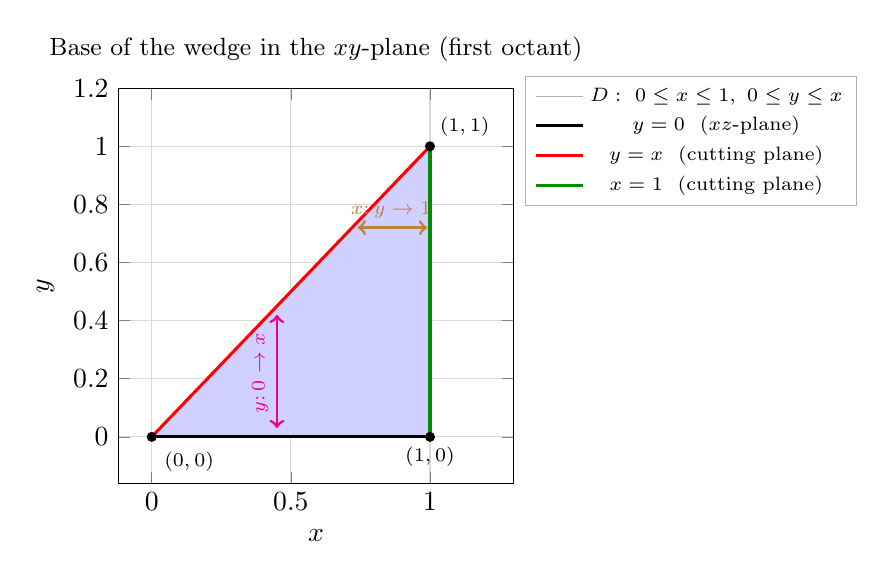
\begin{tikzpicture}
\begin{axis}[
    width=6.6cm, height=6.6cm,
    xmin=-0.12, xmax=1.30, ymin=-0.16, ymax=1.20,
    xlabel=$x$, ylabel=$y$,
    grid=major, grid style={black!15},
    title={Base of the wedge in the $xy$-plane (first octant)},
    title style={font=\small},
    legend style={at={(1.03,1.03)}, anchor=north west, font=\scriptsize,
                  fill=white, draw=black!30}]
    \addplot[fill=blue!18, draw=none] coordinates {(0,0) (1,0) (1,1)};
    \addlegendentry{$D:\ 0\le x\le 1,\ 0\le y\le x$}
    \addplot[black, line width=1.1pt] coordinates {(0,0) (1,0)};
    \addlegendentry{$y=0$ \ ($xz$-plane)}
    \addplot[red, line width=1.1pt, domain=0:1, samples=2] {x};
    \addlegendentry{$y=x$ \ (cutting plane)}
    \addplot[green!55!black, line width=1.1pt] coordinates {(1,0) (1,1)};
    \addlegendentry{$x=1$ \ (cutting plane)}
    \draw[magenta, line width=1pt, <->] (0.45,0.03) -- (0.45,0.42);
    \node[font=\scriptsize, text=magenta, rotate=90] at (axis cs:0.39,0.22) {$y\colon 0\to x$};
    \draw[brown, line width=1pt, <->] (0.74,0.72) -- (0.99,0.72);
    \node[font=\scriptsize, text=brown] at (axis cs:0.86,0.78) {$x\colon y\to 1$};
    \addplot[only marks, mark=*, mark size=1.6pt, black] coordinates {(0,0) (1,0) (1,1)};
    \node[font=\scriptsize, anchor=north west] at (axis cs:0.01,-0.02) {$(0,0)$};
    \node[font=\scriptsize, anchor=north] at (axis cs:1,0) {$(1,0)$};
    \node[font=\scriptsize, anchor=south west] at (axis cs:1,1) {$(1,1)$};
\end{axis}
\end{tikzpicture}
\end{document}
